\scanpage{203}
\figure{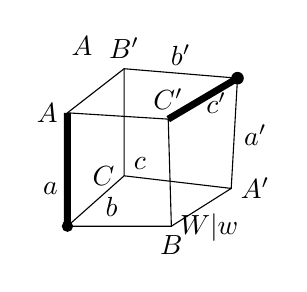
\begin{tikzpicture}[scale=.8]
\draw (0,1.8)--(1.6,1.7)--(1.65,0)--(0,0)--cycle;
\draw (.9,2.5)--(2.7,2.35)--(2.6,.6)--(.9,.8)--cycle;
\draw (0,1.8)--(.9,2.5) (1.6,1.7)--(2.7,2.35) (1.65,0)--(2.6,.6) (0,0)--(.9,.8);
\draw[line width=2.5pt] (0,0)--(0,1.8) (1.6,1.7)--(2.7,2.35);
\fill (0,0) circle(.09);\fill (2.7,2.35) circle(.1);
\node[left] at (0,1.8) {$A$};\node[left] at (0,.6) {$a$};
\node[above] at (.7,0) {$b$};\node[below] at (1.65,0) {$B$};
\node[right] at (2.6,.6) {$A'$};\node[right] at (2.65,1.45) {$a'$};
\node[above] at (1.8,2.4) {$b'$};\node[above] at (.9,2.5) {$B'$};
\node[above left] at (.55,2.55) {$\deleted{\unsure{A}}$};
\node[above] at (1.6,1.7) {$C'$};\node[right] at (2.05,1.95) {$c'$};
\node[left] at (.9,.8) {$C$};\node[above] at (1.15,.75) {$c$};
\node[below] at (2.25,.35) {$\unsure{W|w}$};
\end{tikzpicture}}
\margin{\figure{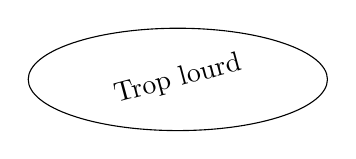
\begin{tikzpicture}\draw (0,0) ellipse (1.9 and .65);
\node[rotate=15] at (0,0) {Trop lourd};\end{tikzpicture}}}
\[
\begin{gathered}
\Sigma_a\quad\Sigma_b\quad\Sigma_c\quad\Sigma_{AB'}\quad
\unsure{\Sigma_{BA'}|\Sigma_{BC'}}\quad\Sigma_{CB'}\quad\Sigma_{CA'}\quad\Sigma_{AC'}\\
\Sigma_{a'}\quad\Sigma_{b'}\quad\Sigma_{c'}
\end{gathered}
\]
\figure{\begin{tikzpicture}
\node[anchor=north west,inner sep=0] at (0,0) {\diagram{\begin{tikzcd}[ampersand replacement=\&, row sep=.6em,column sep=large]
\Sigma_a+\Sigma_{c'}=\Sigma_{AB'}+\Sigma_{BC'}\\
\Sigma_a+\Sigma_{b'}=\Sigma_{AC'}+\Sigma_{CB'}\\
\Sigma_b+\Sigma_{a'}=\Sigma_{BC'}+\Sigma_{CA'}\\
\Sigma_b+\Sigma_{c'}=\Sigma_{BA'}+\Sigma_{AC'}\\
\Sigma_c+\Sigma_{b'}=\Sigma_{CA'}+\Sigma_{AB'}\\
\Sigma_c+\Sigma_{a'}=\Sigma_{CB'}+\Sigma_{BA'}\\[.8em]
\Sigma_a+\Sigma_{CA'}=\Sigma_b+\Sigma_{CB'}\ .\\
\Sigma_{a'}+\Sigma_{AC'}=\Sigma_{b'}+\Sigma_{BC'}\\
\Sigma_b+\Sigma_{AB'}=\Sigma_c+\Sigma_{AC'}\ .\\
\Sigma_{b'}+\Sigma_{BA'}=\Sigma_{c'}+\Sigma_{CA'}\\[.6em]
\Sigma_c+\Sigma_{BC'}=\Sigma_a+\Sigma_{BA'}\ .\\
\Sigma_{c'}+\Sigma_{CB'}=\Sigma_{a'}+\Sigma_{AB'}
\end{tikzcd}}};
\draw (8.0,-.05)..controls (8.25,-.6) and (8.1,-1.0)..(7.8,-1.45)
 ..controls (8.35,-1.9) and (8.3,-2.45)..(7.9,-2.9);
\draw (7.85,-.7)..controls (8.65,-1.2) and (8.55,-1.8)..(7.85,-2.15)
 ..controls (8.8,-2.65) and (8.6,-3.4)..(8.05,-3.55);
\draw (-.25,-.15)..controls (-.15,-2) and (-.05,-3.8)..(-.55,-4.1)
 ..controls (-.05,-4.25) and (-.15,-6.5)..(-.1,-8.65);
\draw[very thick] (.15,-4.55)--(-.02,-4.55)--(-.02,-7.2)--(.15,-7.2);
\end{tikzpicture}}
\margin{$\exists\sigma$ avec
\[\sigma_{\uline{a}}+\sigma_{\uline{b}}+\sigma_{\uline{c}}=\sigma\]
$\forall$ triples d'arêtes formant un ``demi hexagone''
\figure{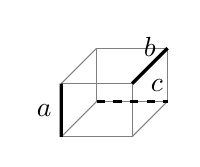
\begin{tikzpicture}[scale=.45]
\draw[gray] (0,0)--(0,1.5)--(2,1.5)--(2,0)--cycle;
\draw[gray] (1,1)--(1,2.5)--(3,2.5)--(3,1)--cycle;
\draw[gray] (0,0)--(1,1) (0,1.5)--(1,2.5) (2,1.5)--(3,2.5) (2,0)--(3,1);
\draw[very thick] (0,0)--(0,1.5) (2,1.5)--(3,2.5);
\draw[dashed,very thick] (1,1)--(3,1);
\node[left] at (0,.75) {$\uline{a}$};\node[above] at (2.5,2) {$\uline{b}$};
\node[above] at (2.7,1) {$\uline{c}$};\end{tikzpicture}}
\[\Sigma_{a'}+\Sigma_{AC'}=\Sigma_{b'}+\Sigma_{BC'}\]}
\margin{chacune des six dernières relations est conséquence des cinq autres,
comme on voit en sommant, \unsure{qui|que} donne $0=0$ !}
\[
\begin{aligned}
&3(\Sigma_a\unsure{+|-}\Sigma_b\unsure{+|-}\Sigma_c+\Sigma_{a'}
 \unsure{+|-}\Sigma_{b'}+\Sigma_{c'})
 +(\Sigma_{CA'}+\Sigma_{AC'}\;\text{---}\;\text{---})\\
&=(\Sigma_a+\Sigma_b\unsure{+|-}\Sigma_c\unsure{+|-}\Sigma_{a'}
 \unsure{+|-}\Sigma_{b'}\unsure{+|-}\Sigma_{c'})+3(\Sigma_{CA'}+\Sigma_{AC'})
\end{aligned}
\]
\margin{202}
